% Compile: pdflatex -interaction=nonstopmode -halt-on-error presentation.tex
\documentclass[aspectratio=169,t]{beamer}
\usetheme{rbras}
\usepackage{amsmath,amssymb}
\renewcommand\tamTituloAbertura{\fontsize{31bp}{36bp}\selectfont}
\renewcommand\tamMensagem{\fontsize{34bp}{42bp}\selectfont}
\title{Inferência causal em dados funcionais via transformadas de ondaletas: do pré-processamento à estimação em tempo real}
\author{\textbf{Moisés Augusto da Silva} · Alex Rodrigo dos Santos Sousa}
\institute{Instituto de Matemática, Estatística e Computação Científica · UNICAMP}
\date{23 de novembro de 2026}
\evento{70\textsuperscript{a} RBras · Concurso de Melhor Dissertação}
\local{Universidade Estadual de Campinas - Campinas - SP}
\emailautor{moisesaugusto@protonmail.com}
\logoevento{logo-rbras.png}
\logoinstituicao{logo-imecc-official.png}
\qrlink{https://github.com/mkyou/rLifting}
\qrlegenda{rLifting: código e documentação}
\begin{document}
\slideabertura
\begin{frame}{Introdução}
\begin{topicos}
\item Intersecção entre inferência causal {\tamLegenda (Rubin, 1974)} e análise de dados funcionais {\tamLegenda (Ramsay e Silverman, 2005)}.
\item Interesse em desfechos funcionais com domínio temporal.
\item Exemplos:
  \begin{itemize}
  \item Consumo de energia elétrica de um domicílio ao longo do ano.
  \item Efeito da dipirona sobre a frequência cardíaca de pessoas alérgicas após a ingestão.
  \end{itemize}
\end{topicos}
\end{frame}
\begin{frame}{Introdução}{Estrutura dos dados}
\begin{columns}[T,onlytextwidth]
\begin{column}{0.48\textwidth}
{\tamCorpo Para cada unidade $i=1,\ldots,N$:\par}
\begin{topicos}
\item Tratamento binário $A_i$, atribuído uma vez.
\item Covariáveis escalares pré-tratamento $\mathbf X_i$.
\item Desfechos potenciais funcionais $Y_i^{(1)}(t)$ e $Y_i^{(0)}(t)$.
\end{topicos}
\end{column}
\begin{column}{0.51\textwidth}
\centering
\begin{tikzpicture}[x=1bp,y=1bp,>=latex,thick,
  obs/.style={circle,draw=rbAzul,minimum size=35bp,inner sep=2bp,font=\tamLegenda},
  est/.style={rectangle,draw=rbAzul,rounded corners=3bp,fill=rbFundo,inner sep=5bp,align=center,font=\tamLegenda}]
\node[obs] (a) at (180,205) {$A_i$};
\node[obs] (ym) at (55,140) {$Y_{i,k-1}$};
\node[obs] (y) at (180,140) {$Y_{i,k}$};
\node[obs] (yp) at (305,140) {$Y_{i,k+1}$};
\draw[->] (ym)--(y); \draw[->] (y)--(yp);
\draw[->] (a)--(y); \draw[->] (a) to[bend left=24] (yp);
\node[est] (on) at (100,40) {$\hat\theta_k$ sequencial};
\node[est] (off) at (275,40) {$\hat\theta_k$ em lote};
\draw[->,rbCinza] (ym)--(on); \draw[->,rbCinza] (y)--(on);
\draw[->,rbCinza] (y)--(off); \draw[->,dashed,rbAzul] (yp)--(off);
\end{tikzpicture}\par
{\tamLegenda Dependência de observações futuras: linha tracejada.\\Adaptado da Figura 21 da dissertação.\par}
\end{column}
\end{columns}
\end{frame}
\begin{frame}{Introdução}{FATE e efeito acumulado}
\begin{topicos}
\item O efeito médio de tratamento funcional (FATE), para $t\in\mathcal T$, é definido por Ecker et al. (2024):
\end{topicos}
{\tamEquacao\[
\theta(t)=\mathbb E\!\left[Y_i^{(1)}(t)-Y_i^{(0)}(t)\right].
\]}
\begin{topicos}
\item Propomos o CFATE para quantificar o efeito acumulado desde o instante da intervenção:
\end{topicos}
{\tamEquacao\[
\Theta(t)=\int_{t_{\mathrm{trat}}}^{t}\theta(s)\,ds.
\]}
\end{frame}
\begin{frame}{Suposições de identificação}{Consistência e ausência de interferência}
{\tamCorpo Para $a\in\mathcal A\equiv\{0,1\}$ e $t\in\mathcal T$:\par}
\begin{topicos}
\item Consistência: se $A_i=a$, a trajetória observada é o desfecho potencial sob $a$:
\end{topicos}
{\tamEquacao\[
Y_i(t)=A_iY_i^{(1)}(t)+(1-A_i)Y_i^{(0)}(t).
\]}
\begin{topicos}
\item Ausência de interferência: o tratamento atribuído a outra unidade $j\ne i$ não afeta $Y_i^{(a)}(t)$.
\item Em conjunto, constituem a SUTVA: Suposição de Valor de Tratamento de Unidade Estável.
\end{topicos}
\end{frame}
\begin{frame}{Suposições de identificação}{Positividade e ignorabilidade média}
{\tamCorpo Para $a\in\mathcal A=\{0,1\}$ e todo $t\in\mathcal T$:\par}
\vspace{4bp}
{\tamEquacao\[
0<\pi_a(\mathbf X_i)=\mathbb P(A_i=a\mid\mathbf X_i)<1\quad\text{q.c.}
\]}
{\tamCorpo Ambos os tratamentos são possíveis para cada perfil de covariáveis.\par}
\vspace{12bp}
{\tamEquacao\[
\mathbb E\!\left[Y_i^{(a)}(t)\mid A_i,\mathbf X_i\right]
=\mathbb E\!\left[Y_i^{(a)}(t)\mid\mathbf X_i\right].
\]}
{\tamCorpo Dadas as covariáveis, a média do desfecho potencial não depende da atribuição observada.\par}
\end{frame}
\begin{frame}{Abordagem de Ecker et al.}{Estimação do FATE}
\begin{topicos}
\item Representam as trajetórias discretas por funções, utilizando suavização por \textit{splines}.
\item Ajustam modelos de regressão linear funcional separadamente para os grupos tratado e controle.
\item Estimam o FATE pela diferença média entre as predições dos dois modelos na amostra.
\item Constroem bandas de confiança simultâneas sob as hipóteses do modelo, incluindo erros gaussianos.
\end{topicos}
\end{frame}
\begin{frame}{Estimação do FATE}{Proposta}
\begin{columns}[T,onlytextwidth]
\begin{column}{0.36\textwidth}
\begin{topicos}
\item Ondaletas no pré-processamento, acomodando irregularidades locais {\tamLegenda (Mallat, 1989; Sweldens, 1995)}.
\item \textsf{rLifting}: R/C++, processamento em lote e sequencial, com suporte a grades irregulares {\tamLegenda (inspirado em Liu et al., 2014)}.
\end{topicos}
\end{column}
\begin{column}{0.62\textwidth}
{\tamCorpoDois Comparação de suavização em lote\par}
\vspace{10bp}
{\tamLegenda\renewcommand\arraystretch{1.55}
\begin{tabularx}{\linewidth}{@{}l *{4}{>{\raggedleft\arraybackslash}X}@{}}
\toprule
& \multicolumn{2}{c}{Regular} & \multicolumn{2}{c}{Irregular}\\
Pacote & Tempo & MG-MSE & Tempo & MG-MSE\\
\midrule
rLifting & 0,080 & 0,0113 & 0,152 & 0,0087\\
wavethresh & 3,199 & 0,0096 & --- & ---\\
adlift & 3.006,222 & 0,0108 & 3.233,967 & 0,0068\\
nlt & 3.628,600 & 0,0150 & 2.922,728 & 0,0104\\
\bottomrule
\end{tabularx}\par}
\vspace{12bp}
{\tamLegenda Tempo mediano em $\mu$s por amostra; MG-MSE: média geométrica das medianas dos MSEs. Melhor configuração de cada pacote por sinal.\par\vspace{5bp}Grade regular: quatro sinais; irregular: sete sinais. $T=1{.}024$ e $1{.}000$ réplicas por configuração. O \textsf{wavethresh} requer grade uniforme.\par}
\end{column}
\end{columns}
\end{frame}
\begin{frame}{Estimação do FATE}{Em lote e sequencial}
\begin{topicos}
\item Como em Ecker et al., estimamos o FATE por regressões separadas por grupo:
\end{topicos}
\vspace{8bp}
{\tamEquacao\[
\hat\theta(t)=\bar{\mathbf X}^{\mathsf T}\!\left(\hat{\boldsymbol\beta}^{(1)}(t)-\hat{\boldsymbol\beta}^{(0)}(t)\right).
\]}
\vspace{8bp}
\begin{topicos}
\item Em lote: pré-processamos a trajetória completa.
\item Sequencial: pré-processamos uma janela de observações disponíveis até o instante corrente.
\item CFATE estimado: integramos o FATE pela regra do trapézio.
\end{topicos}
\end{frame}
\begin{frame}{Estimação do FATE}{Incerteza}
\begin{topicos}
\item A limiarização por ondaletas é uma operação não linear; as bandas analíticas de Ecker et al. não se aplicam diretamente.
\item Usamos \textit{bootstrap} não paramétrico para construir bandas de confiança simultâneas.
\item Reamostramos indivíduos com suas trajetórias completas e ajustamos os modelos às réplicas sem pré-processamento.
\end{topicos}
\end{frame}
\begin{frame}{Simulações}{Desenhos de experimento}
\begin{topicos}
\item Desenho comum: nove covariáveis, atribuição logística e erros gaussianos ou $t$-Student(5):
\end{topicos}
{\tamEquacao\[
\operatorname{logit}\!\bigl[\mathbb P(A_i=1\mid\mathbf X_i)\bigr]
=\gamma_0+\mathbf X_i^{\mathsf T}\boldsymbol\gamma,\qquad
Y_i^{(1)}(t)-Y_i^{(0)}(t)=\frac{\delta(t)}{10}\!\left(1+\sum_{k=1}^{9}X_{ik}\right).
\]}
\begin{topicos}
\item Simulação 1: comparação com \textit{splines} e omissão de confundidoras nas ondaletas.
\item Simulação 2: estimação sequencial ponto a ponto e latência.
\item Simulação 3: três graus de irregularidade da grade temporal.
\end{topicos}
\end{frame}
\begin{frame}{Simulações}{Resultados por cenário}
{\tamLegenda\renewcommand\arraystretch{1.55}\setlength{\tabcolsep}{4bp}
\resizebox{\linewidth}{!}{%
\begin{tabular}{@{}lccccccccccc@{}}
\toprule
& \multicolumn{6}{c}{Simulação 1} & Simulação 2 & \multicolumn{4}{c}{Simulação 3}\\
\cmidrule(lr){2-7}\cmidrule(lr){8-8}\cmidrule(l){9-12}
& \multicolumn{3}{c}{NRMSE (cobertura)} & \multicolumn{3}{c}{Cobertura: omissão} & Latência & \multicolumn{4}{c}{NRMSE (cobertura): grade}\\
Cenário & Lote & Seq. & Ecker & Baixa & Média & Alta & ($\mu$s) & Uniforme & Leve & Moderada & Severa\\
\midrule
Sigmoide & 0,011 (95,3) & 0,010 (94,2) & 0,030 (0,0) & 91,5 & 83,7 & 26,8 & 9,52 & 0,010 (94,2) & 0,011 (93,6) & 0,010 (96,1) & 0,010 (94,9)\\
\textit{Bumps} & 0,001 (95,8) & 0,001 (94,6) & 0,046 (0,0) & 93,6 & 33,8 & 0,3 & 10,43 & 0,001 (94,6) & 0,001 (93,9) & 0,001 (94,2) & 0,001 (95,0)\\
\textit{Doppler} & 0,008 (94,9) & 0,022 (94,4)$^*$ & 0,003 (0,0) & 94,0 & 92,3 & 97,7 & 10,35 & 0,022 (94,4) & 0,022 (95,9) & 0,012 (95,0) & 0,012 (95,7)\\
Escada & 0,001 (94,4) & 0,001 (94,3) & 0,055 (0,0) & 86,8 & 4,7 & 0,5 & 9,60 & 0,001 (94,3) & 0,001 (94,7) & 0,001 (94,9) & 0,001 (93,5)\\
\bottomrule
\end{tabular}}\par}
\vspace{12bp}
{\tamLegenda $N=2.000$, $T=512$ e erros gaussianos. Coberturas simultâneas do FATE (\%), nominais de 95\%. Omissão e grade: estimador sequencial; grade uniforme: Simulação 1. Latência média de suavização por indivíduo e instante; não inclui a estimação do FATE.\par\vspace{5bp}$^*$ Em estudos menores realizados após a dissertação, notamos que o emprego de ondaletas mais adequadas para o cenário \textit{Doppler} diminuiu o NRMSE para 0,003.\par}
\end{frame}
\begin{frame}{Aplicação: Low Carbon London}{Dados e desenho}
\begin{topicos}
\item $N=5.095$ domicílios; consumo elétrico registrado a cada 30 minutos durante 2013 ($T=17.520$).
\item Tratamento: tarifa dinâmica; controle: tarifa padrão.
\item Atribuição aleatorizada por estratos socioeconômicos ACORN, incluídos como covariáveis.
\item Estimamos o FATE e o CFATE usando ondaletas em lote e sequenciais.
\end{topicos}
\end{frame}
\begin{frame}{Aplicação: Low Carbon London}{Resultados}
\begin{columns}[T,onlytextwidth]
\begin{column}{0.32\textwidth}
\centering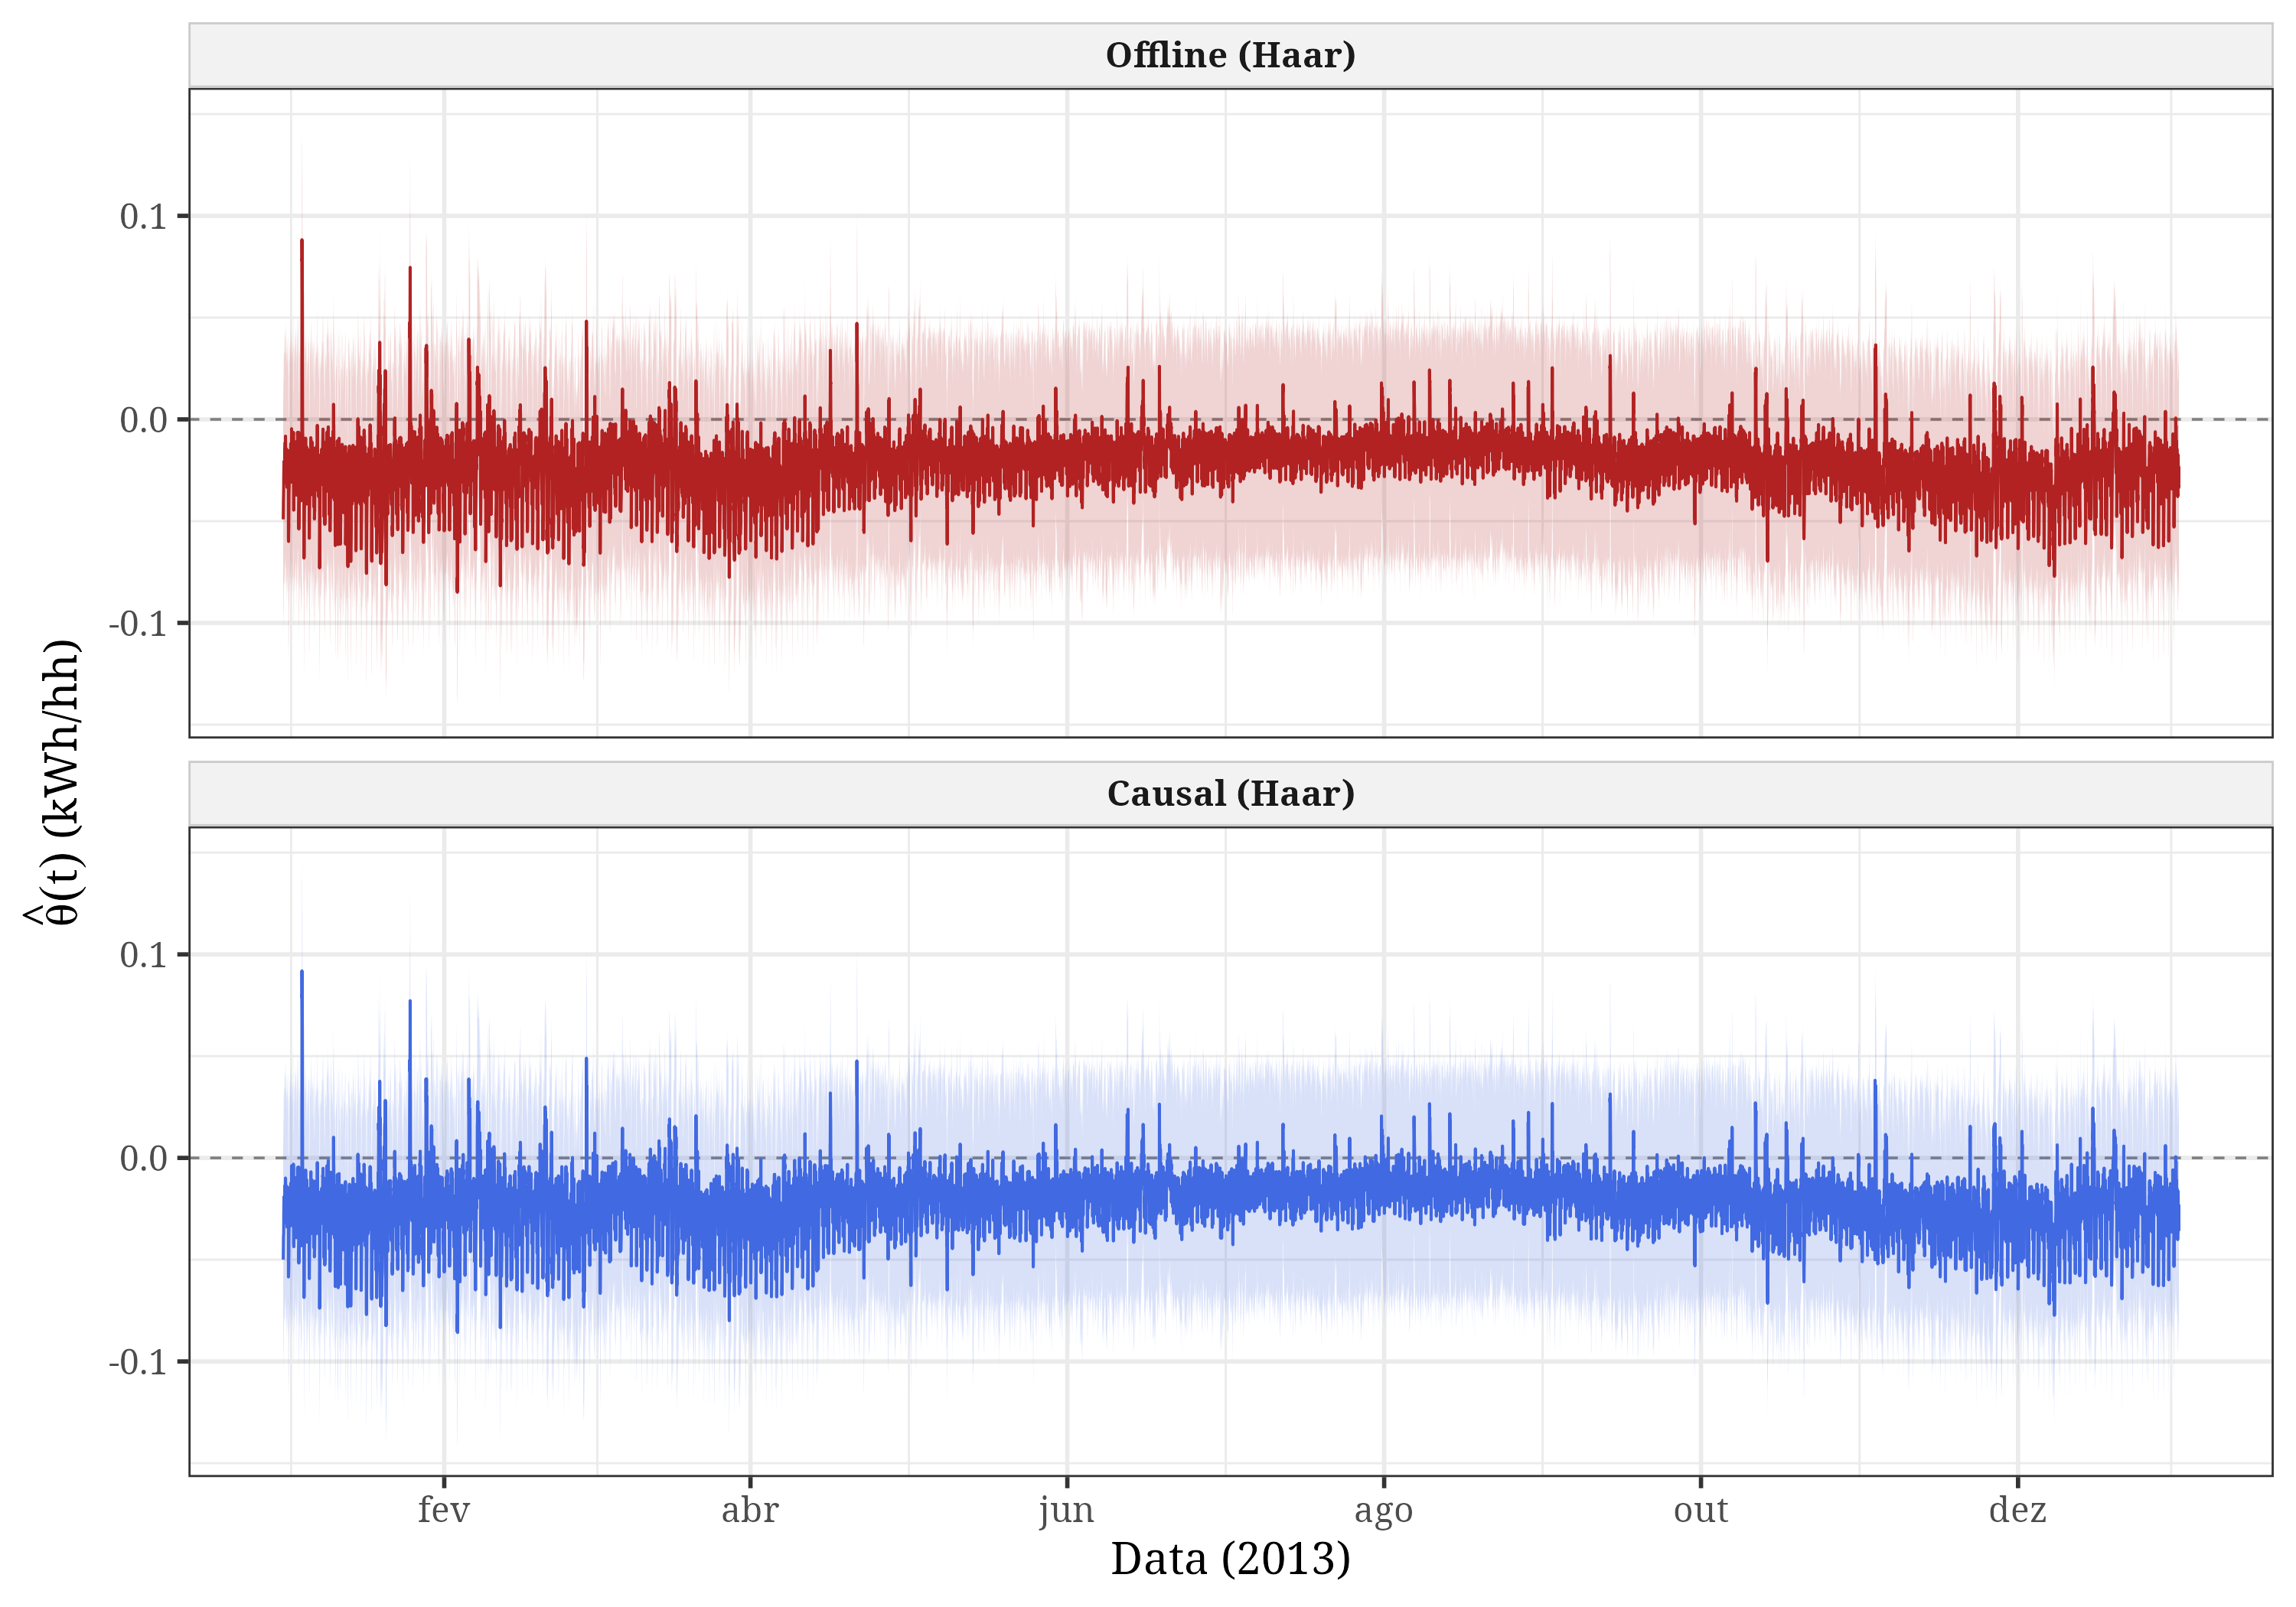
\includegraphics[width=\linewidth]{figures/fate_bands.png}\par
{\tamLegenda FATE: efeito médio em cada intervalo de 30 minutos.\par}
\end{column}
\begin{column}{0.32\textwidth}
\centering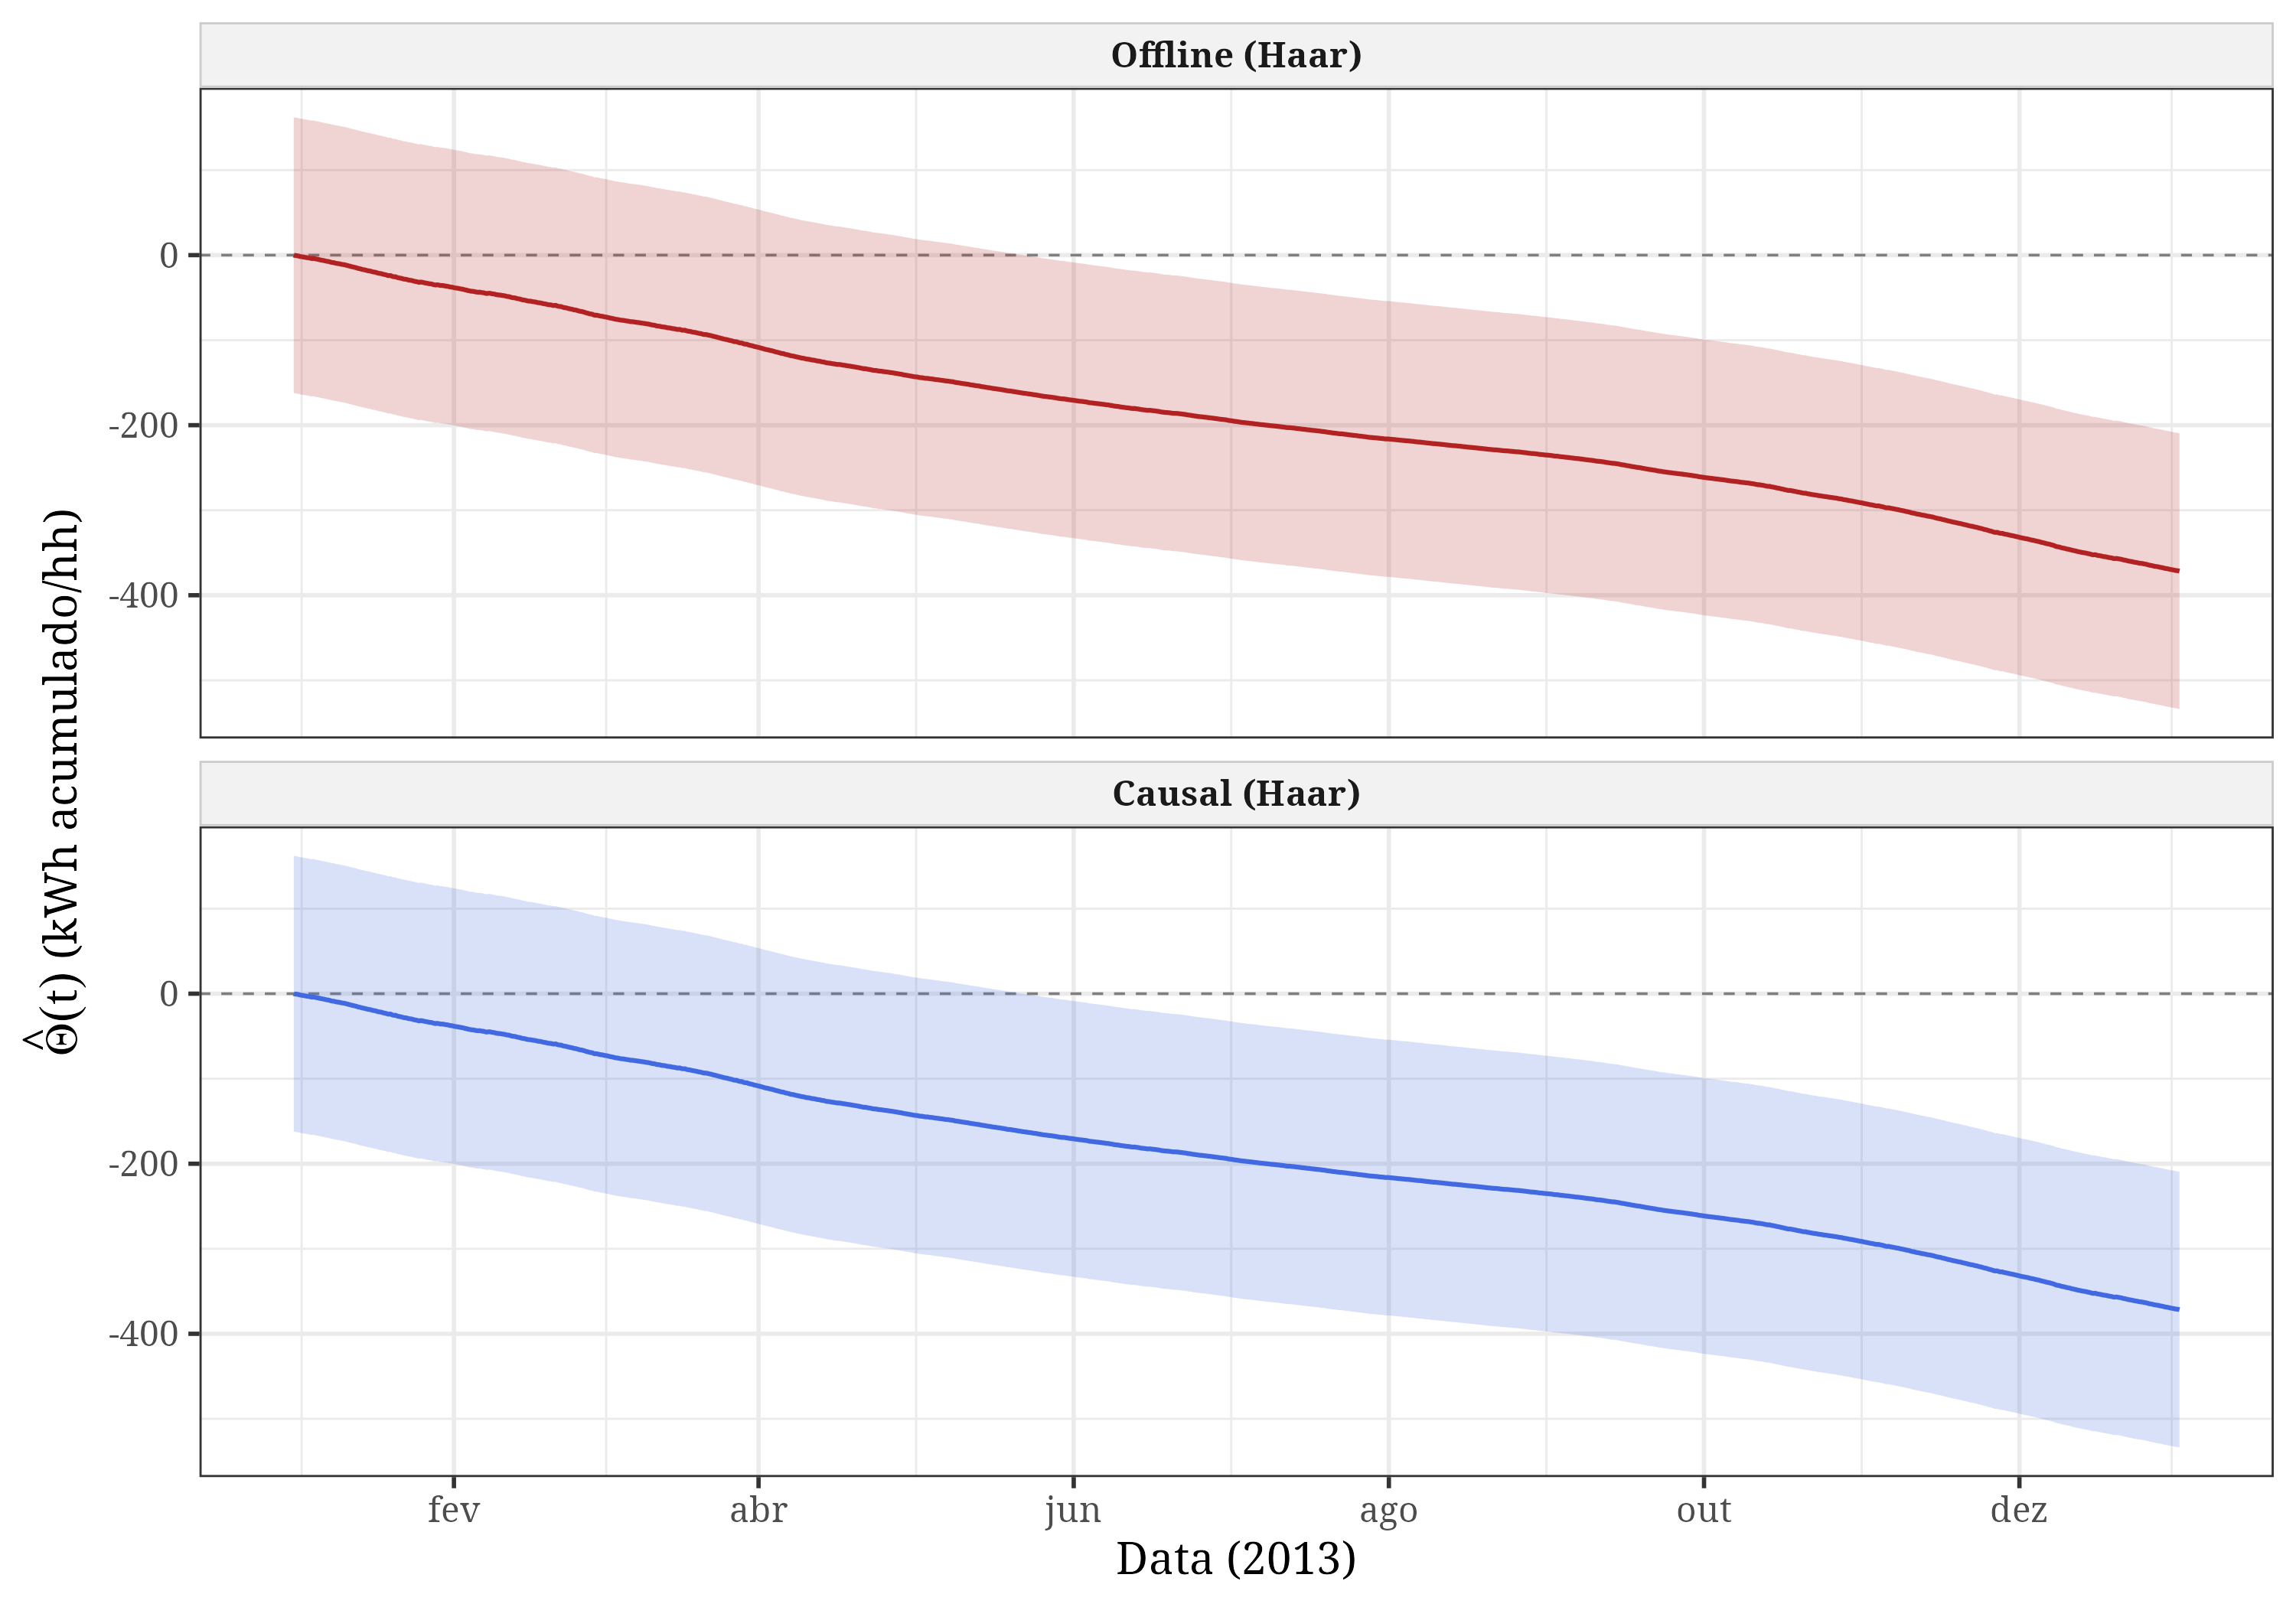
\includegraphics[width=\linewidth]{figures/cfate_annual.png}\par
{\tamLegenda CFATE: efeito médio acumulado ao longo de 2013.\par}
\end{column}
\begin{column}{0.34\textwidth}
\centering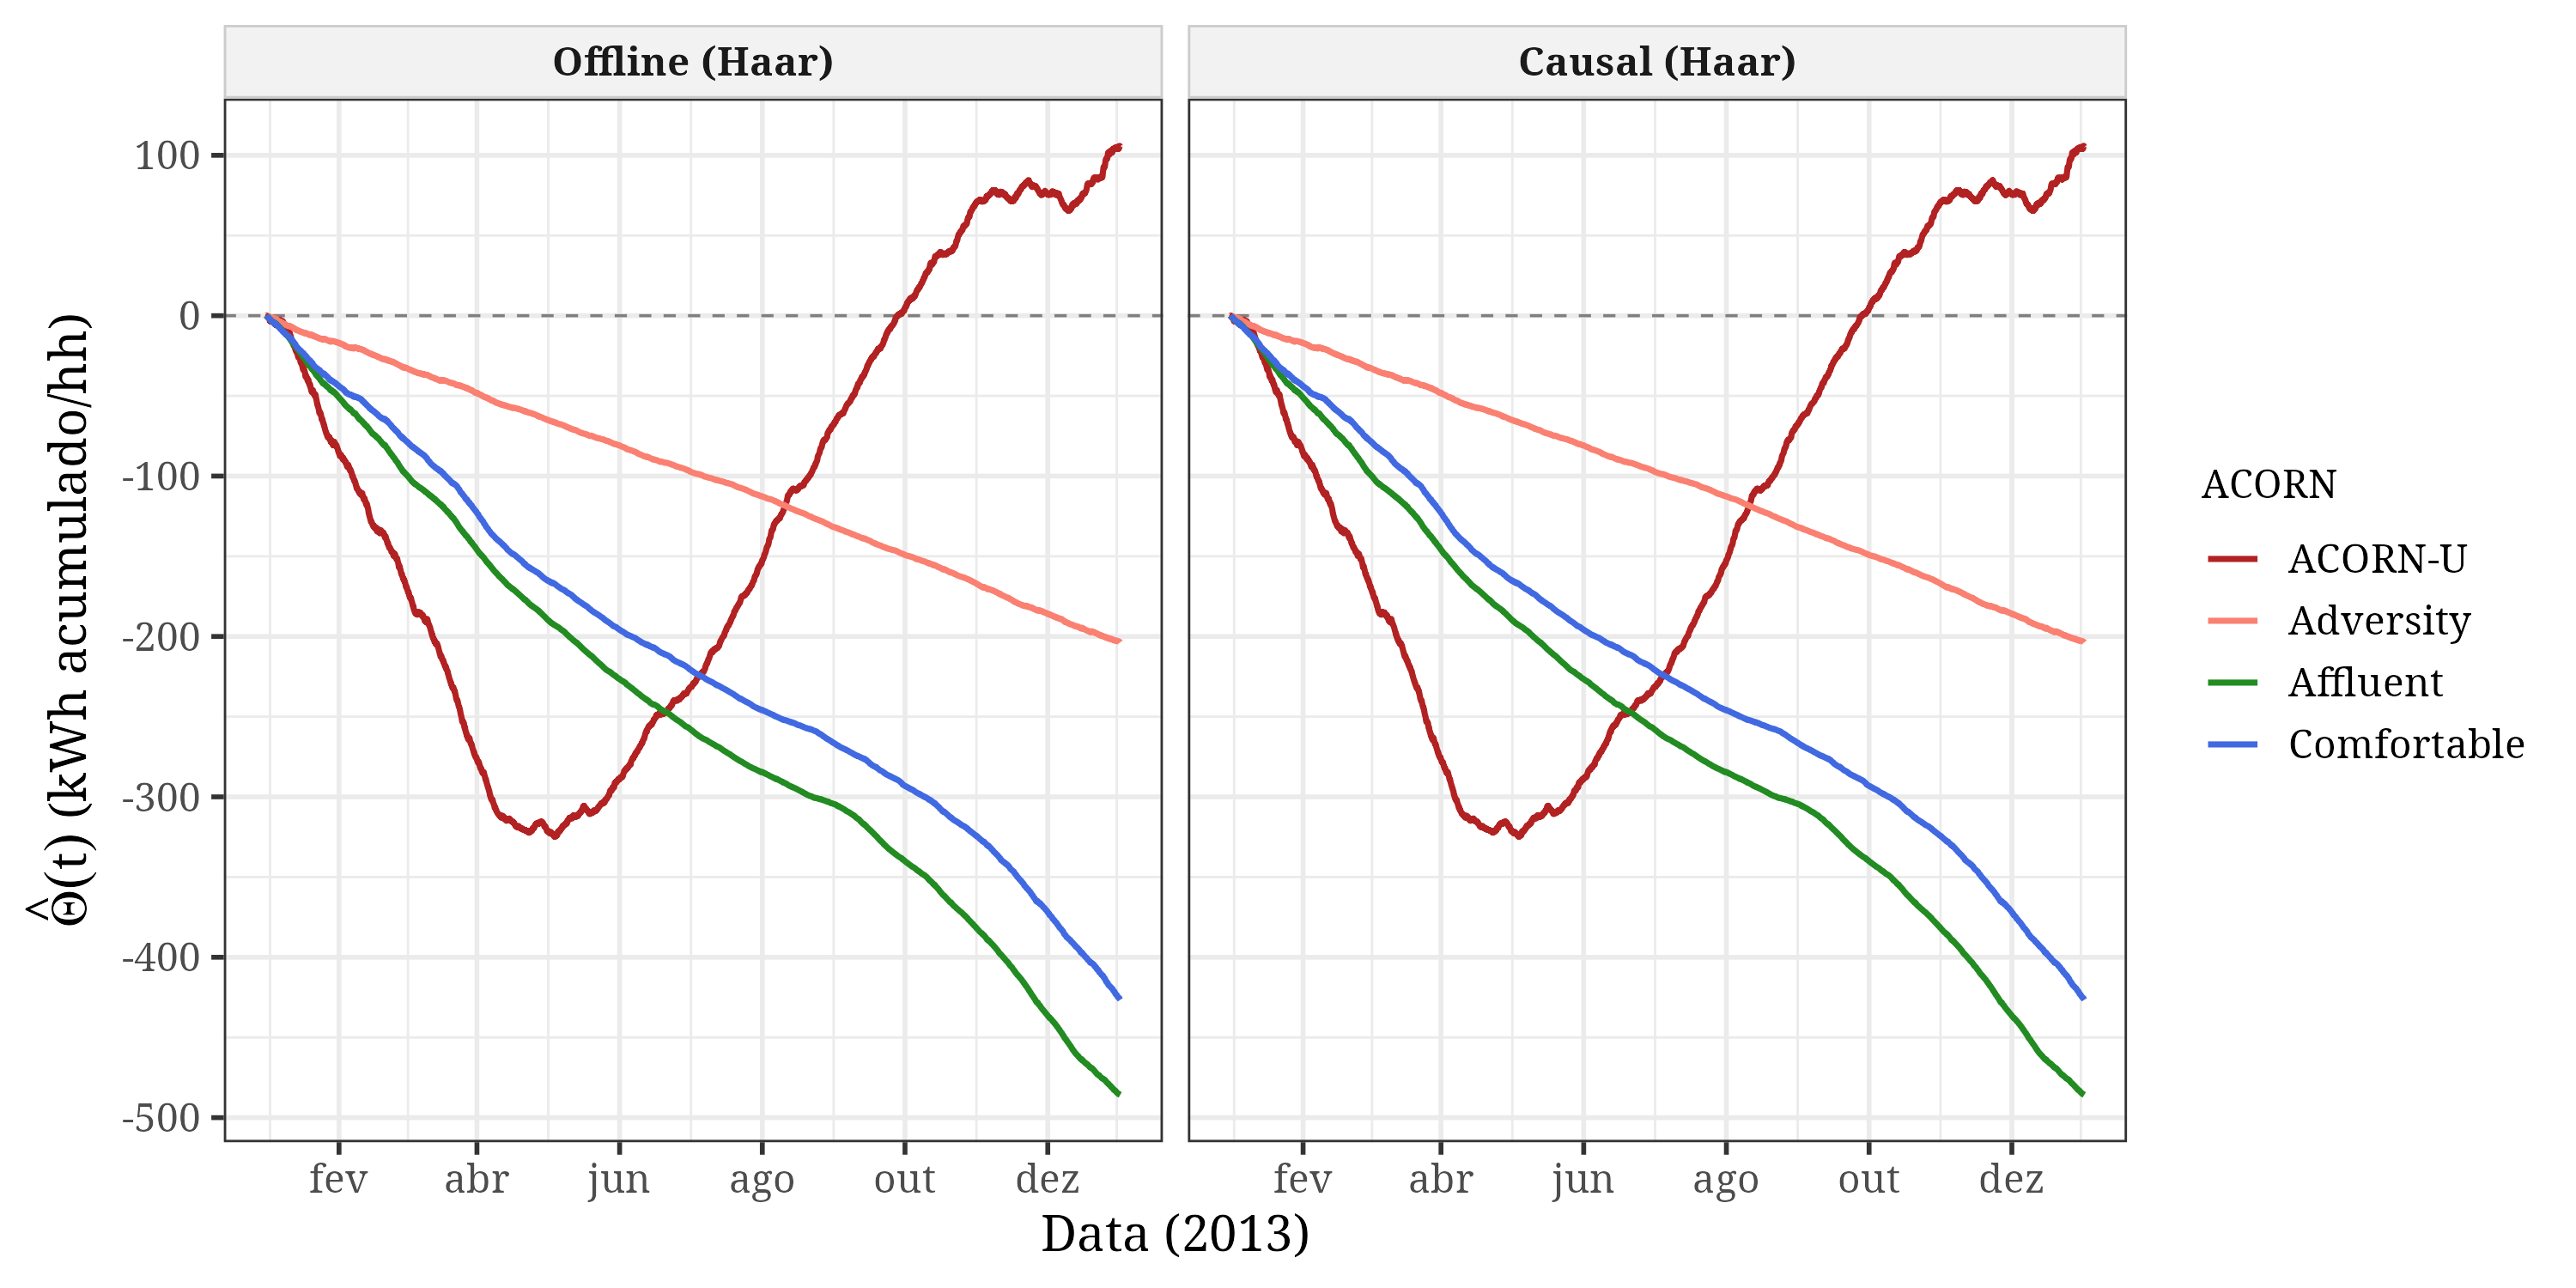
\includegraphics[width=\linewidth,height=0.7\linewidth]{figures/cfate_by_acorn.png}\par
{\tamLegenda CFATE por perfil socioeconômico ACORN.\par}
\end{column}
\end{columns}
\vspace{12bp}
{\tamLegenda Nos dois primeiros gráficos, faixas indicam bandas simultâneas de 95\%; vermelho: em lote, azul: sequencial. No terceiro, as cores identificam os grupos ACORN.\par}
\vspace{8bp}
{\tamCorpoDois CFATE ao fim de 2013: $-372$ kWh por domicílio (IC 95\%: $[-534; -209]$).\par}
\end{frame}
\begin{frame}{Limitações e próximos passos}
\begin{topicos}
\item Relaxar a exigência de uma grade temporal compartilhada entre indivíduos.
\item Incorporar covariáveis variantes no tempo e regimes dinâmicos de tratamento.
\item Relaxar a linearidade do modelo e investigar estimadores duplamente robustos.
\item Estender o pré-processamento a dados multivariados, considerando o custo computacional.
\end{topicos}
\end{frame}
\slideconclusoes
{Ondaletas permitem estimar o FATE sequencial e o CFATE.}
{Simulações indicam bom desempenho também em grades irregulares.}
{Na aplicação, estimamos redução acumulada de $372$ kWh por domicílio.}
\begin{frame}{Referências}
\relax
{\tamLegenda
Rubin, D. B. (1974). Estimating causal effects of treatments in randomized and nonrandomized studies. \textit{Journal of Educational Psychology}, 66, 688--701.\par\vspace{8bp}
Ramsay, J. O.; Silverman, B. W. (2005). \textit{Functional Data Analysis}. 2. ed. Springer.\par\vspace{8bp}
Ecker, K.; De Luna, X.; Schelin, L. (2024). Causal inference with a functional outcome. \textit{Journal of the Royal Statistical Society: Series C}, 73, 221--240.\par\vspace{8bp}
Mallat, S. G. (1989). A theory for multiresolution signal decomposition: the wavelet representation. \textit{IEEE Transactions on Pattern Analysis and Machine Intelligence}, 11, 674--693.\par\vspace{8bp}
Sweldens, W. (1995). Lifting scheme: a new philosophy in biorthogonal wavelet constructions. \textit{Proceedings of SPIE}, 68--79.\par\vspace{8bp}
Liu, Z.; Mi, Y.; Mao, Y. (2014). Improved real-time denoising method based on lifting wavelet transform. \textit{Measurement Science Review}, 14, 152--159.\par\vspace{8bp}
Schofield, J. et al. (2015). \textit{Low Carbon London: Data from the dynamic time-of-use electricity pricing trial, 2013}. UK Data Service.\par}
\end{frame}
\slideencerramento[\inserttitle]
\end{document}
